% ============================================================
% HYPOTHESIS 1 — VERIFICATION
% ============================================================

\section{Hypothesis 1 — Verification}

\begin{frame}{Hypothesis 1: Attention Control}

\textbf{Hypothesis 1:}

Hệ số $d$ điều khiển mức độ đóng góp của retrieved documents vào attention, từ đó ảnh hưởng đến Language Modeling Loss.

\vspace{0.35cm}

\[
A = dA_{\mathrm{doc}} + (1-d)A_{\mathrm{no\_doc}}
\]

\vspace{0.3cm}

\textbf{Verification:}

\begin{itemize}
    \item Cố định question, answer và retrieved documents.
    \item Thay đổi $d \in \{0/32,\ldots,32/32\}$.
    \item Đo và so sánh $L_{\mathrm{LM}}(d)$.
\end{itemize}

\end{frame}

\begin{frame}{Hypothesis 1: Validation Sample}

\textbf{Question}
\begin{quote}
How many times did plague occur in the place where the creator of The Worship of Venus died?
\end{quote}

\textbf{Answer:} 22

\vspace{0.2cm}

\textbf{Golden Passages (3)}
\begin{itemize}
    \item The Martyrdom of Saint Lawrence (Titian)
    \item The Worship of Venus
    \item Black Death
\end{itemize}

\textbf{Distractor Passages (17)}
\begin{itemize}
    \item 2013 Houphouët-Boigny stampede
    \item Peter Strudel
    \item Acral necrosis
    \item Christian Ackermann
    \item Black Death in England
    \item \textit{... and 12 other passages}
\end{itemize}

\end{frame}
\begin{frame}{Hypothesis 1: Validation Pipeline}

\centering

\textbf{One Sample}\\
\small Question + Answer + Golden Passages + Distractors

\vspace{0.2cm}
$\downarrow$

\textbf{Construct Passage Ratios}

\vspace{0.2cm}

\begin{columns}[T,onlytextwidth]
    \column{0.24\textwidth}
    \centering
    \textbf{3:0}\\
    \scriptsize
    The Martyrdom of Saint Lawrence\\
    The Worship of Venus\\
    Black Death

    \column{0.24\textwidth}
    \centering
    \textbf{2:1}\\
    \scriptsize
    The Worship of Venus\\
    Black Death\\
    Peter Strudel

    \column{0.24\textwidth}
    \centering
    \textbf{1:2}\\
    \scriptsize
    Black Death\\
    Peter Strudel\\
    Acral necrosis

    \column{0.24\textwidth}
    \centering
    \textbf{0:3}\\
    \scriptsize
    Peter Strudel\\
    Acral necrosis\\
    Tundra Publishing
\end{columns}

\vspace{0.1cm}
$\downarrow$

\textbf{33 Decision Scores per Ratio}

\[
d \in \{0/32, 1/32, \ldots, 32/32\}
\]

\vspace{0.1cm}
$\downarrow$

\textbf{Measure Language Modeling Loss}
\[
L_{\mathrm{LM}}(d)
\]

\end{frame}

\begin{frame}[fragile]{Hypothesis 1: Prompt Example}

\tiny
\begin{verbatim}
<|im_start|>system
You are a helpful assistant that can solve the given question step by step.
For each step, start by explaining your thought process.
If additional information is needed, the system will perform retrieval and
return the top search results within <observation> and </observation>.
Continue your reasoning using the retrieved information.
When you know the final answer, provide it within <answer> and </answer> tags.
<|im_end|>
<|im_start|>user
How many times did plague occur in the place where the creator of The Worship of Venus died?
<|im_end|>
<|im_start|>assistant
<|im_end|>
<|im_start|>user

<observation>
Title: The Martyrdom of Saint Lawrence (Titian)
The 1558 painting by Titian, now in the church of I Gesuiti in Venice, ...

Title: 2013 Houphouët-Boigny stampede
A fatal stampede in Abidjan, Ivory Coast, resulting in 61 deaths and over 200 injuries, ...

Title: Peter Strudel
An Austrian artist associated with the Academy of Fine Arts Vienna; a plague house
operated there before his death, ...
</observation>
<|im_end|>
<|im_start|>assistant
22<|im_end|>
\end{verbatim}

\end{frame}

\begin{frame}{Hypothesis 1: Validation Results}

\centering

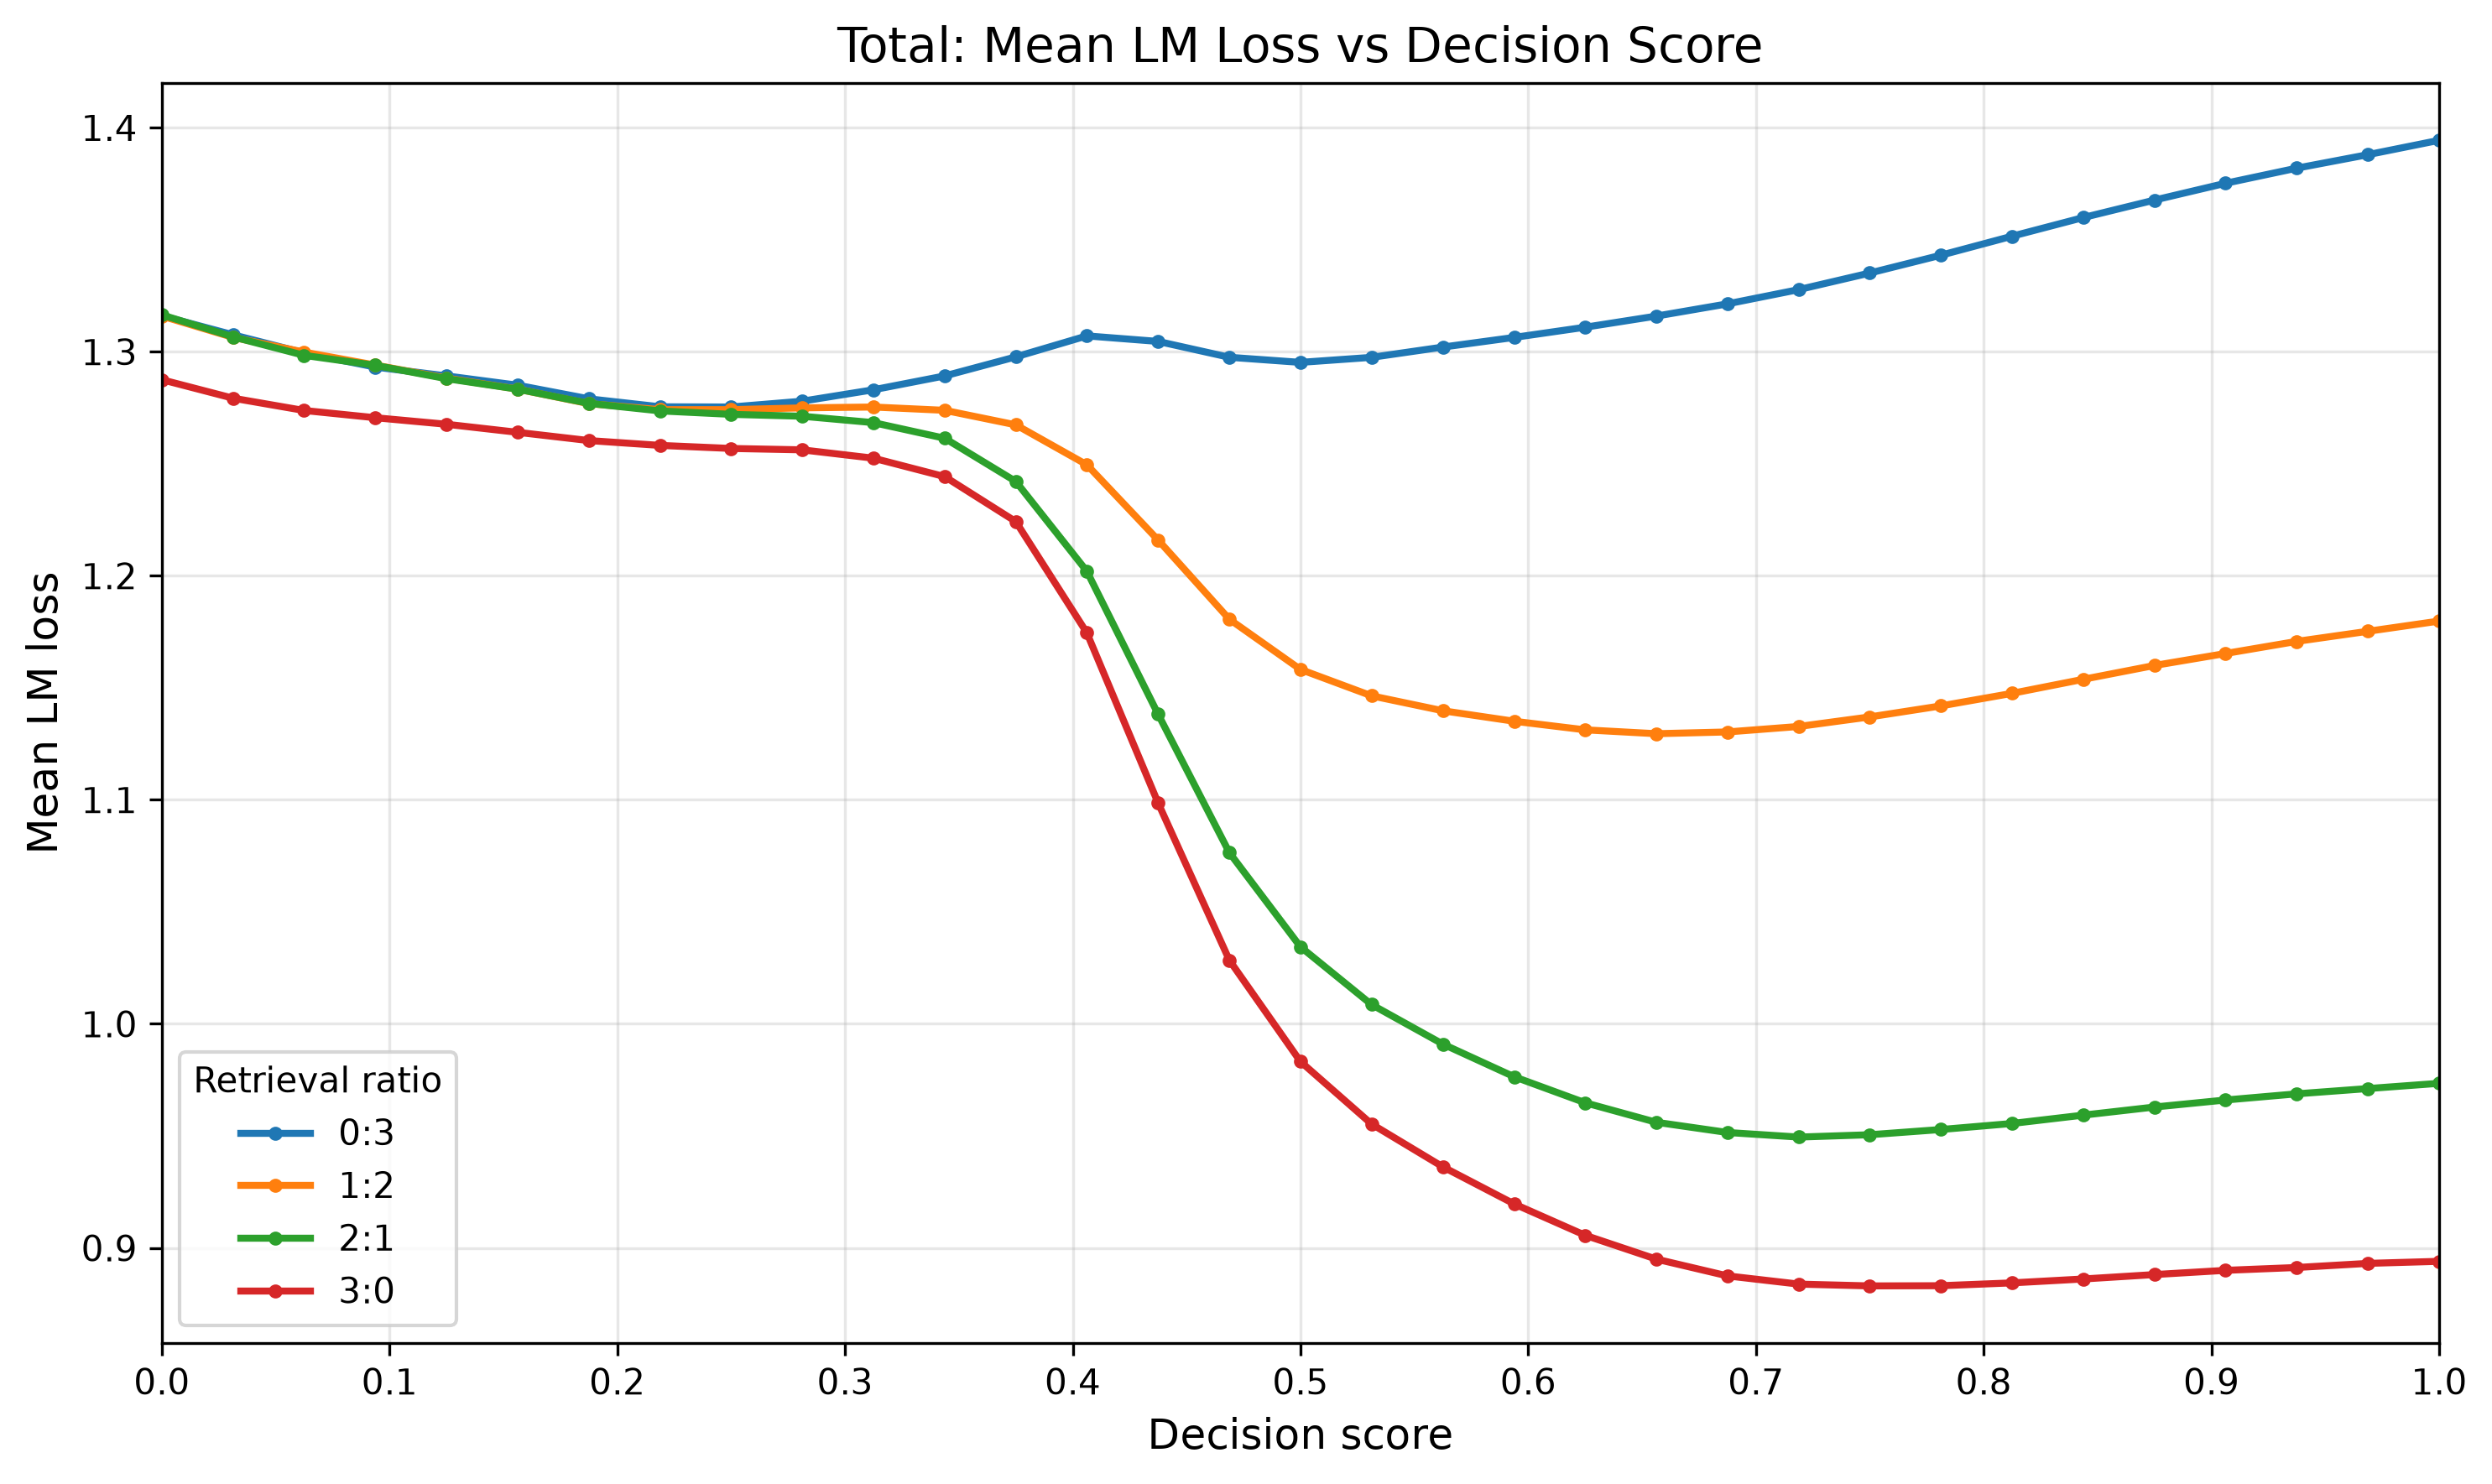
\includegraphics[width=\textwidth,height=0.78\textheight,keepaspectratio]{images/lm_loss_vs_decision_score_total.png}

\end{frame}
